%\Chapter{Results and Discussions}
\Chapter{Results and Conclusions}
\label{chap:results}
    This chapter summarises the results of simulation of entire converter using PID control and current mode control techniques. The experimentation results on the hardware setup are also presented herein.

\section{Simulations}
	The values of components derived in chapter \ref{chap:hardware} are used in a simulation of the converter with 50 kHz switching frequency and 5 kHz machining frequency. Table \ref{tab:sim1-param} enlists the simulation parameters used.
	\begin{comment}
		The voltage and current waveforms across the load when direct duty ratio control is used are shown in figure \ref{fig:1b}. Figure \ref{fig:sim-cmc} shows the load voltage and current waveforms when current mode control is used. The output waveforms thus obtained are in well agreement with the results in \cite{tastekin2009novel}.
		\begin{figure}[H]
			\begin{subfigure}{0.49\textwidth}
				\centering
				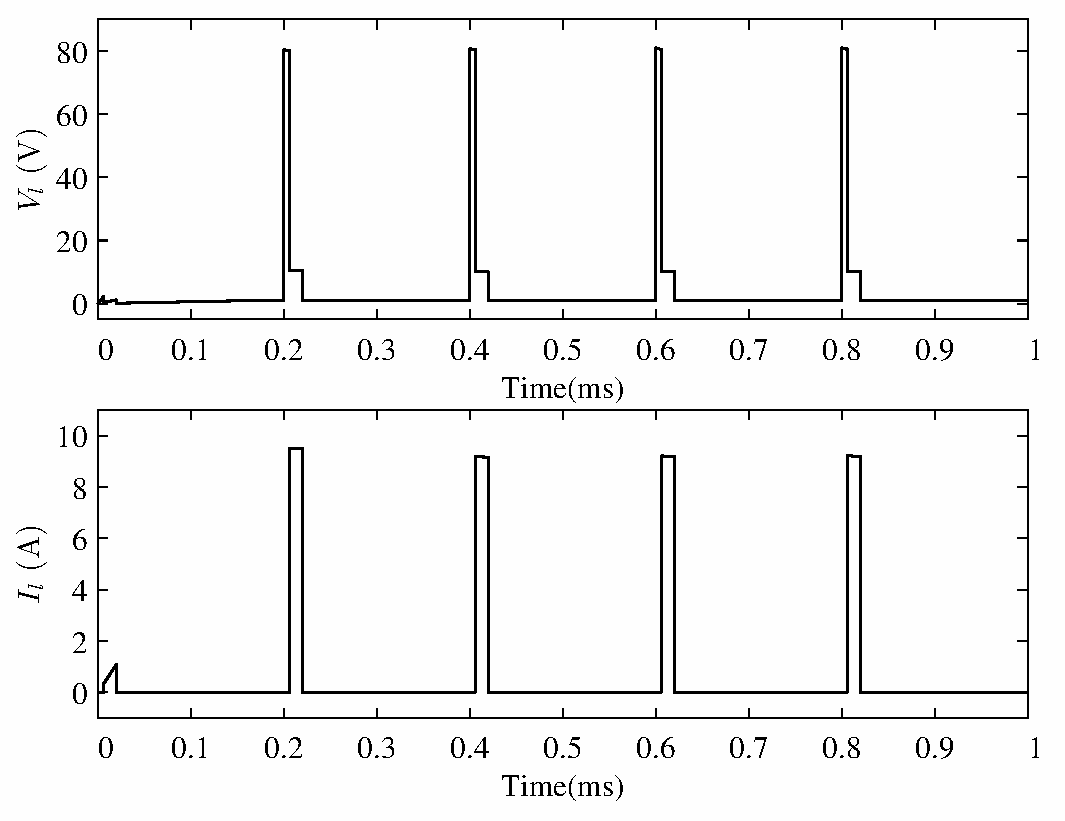
\includegraphics[width=0.95\linewidth]{load_comp}
				\caption{Direct duty ratio control}
				\label{fig:1b}
			\end{subfigure}
			\begin{subfigure}{0.49\textwidth}
				\centering
				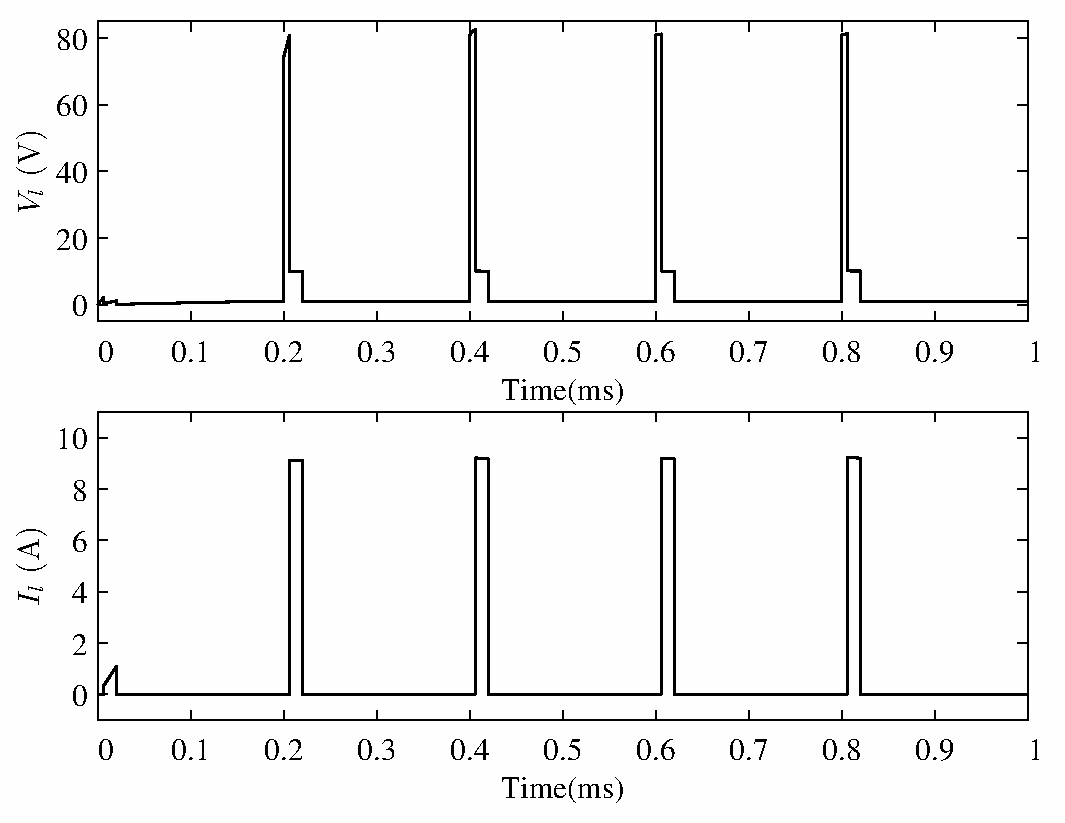
\includegraphics[width=0.95\linewidth]{load_cmc}
				\caption{Current mode control}
				\label{fig:sim-cmc}
			\end{subfigure}
			\caption{Load voltage and current}
		\end{figure}
		Figure \ref{fig:sim-qd} shows the voltage across $Q_d$ and current through $Q_d$ waveforms when direct duty ratio control is used. The maximum voltage across $Q_d$ is $V_{\text{ref}}$ i.e. 80 V and and the maximum current through $Q_d$ is 11 A during the rise time. Figure \ref{fig:sim-d} shows the voltage across $D$ and current through $D$ waveforms when direct duty ratio control is used. The maximum reverse voltage across $D$ is 83 V and the maximum forward current through it is 0.8 A.
		\begin{figure}[H]
			\begin{subfigure}{0.49\textwidth}
				\centering
				\includegraphics[width=0.95\linewidth]{Qd}
				\caption{Voltage and current of Qd}
				\label{fig:sim-qd}
			\end{subfigure}
			\begin{subfigure}{0.49\textwidth}
				\centering
				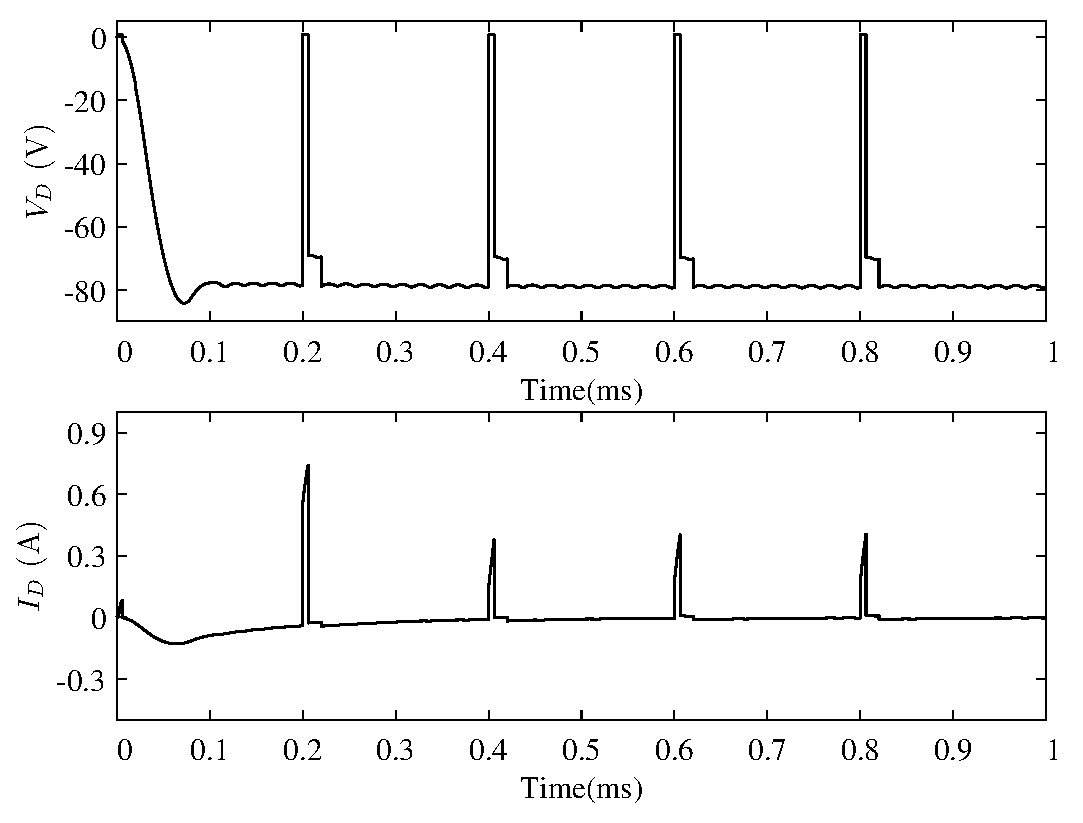
\includegraphics[width=0.95\linewidth]{D}
				\caption{Voltage and current of D}
				\label{fig:sim-d}
			\end{subfigure}
			\caption{Direct duty ratio control: Qd,D}
		\end{figure}
		Figure \ref{fig:sim-q1} shows the voltage across $Q_1$ and current through $Q_1$ waveforms when direct duty ratio control is used. The maximum voltage across $Q_1$ is $V_d$ i.e 110 V and the maximum current through it is 11 A. Figure \ref{fig:sim-d1} shows the voltage across $D_1$ and current through $D_1$ waveforms when direct duty ratio control is used. The maximum reverse voltage across diode $D_1$ is $V_d$ i.e. 110 V and the maximum forward current through it is 11 A.
		\begin{figure}[H]
			\begin{subfigure}{0.49\textwidth}
				\centering
				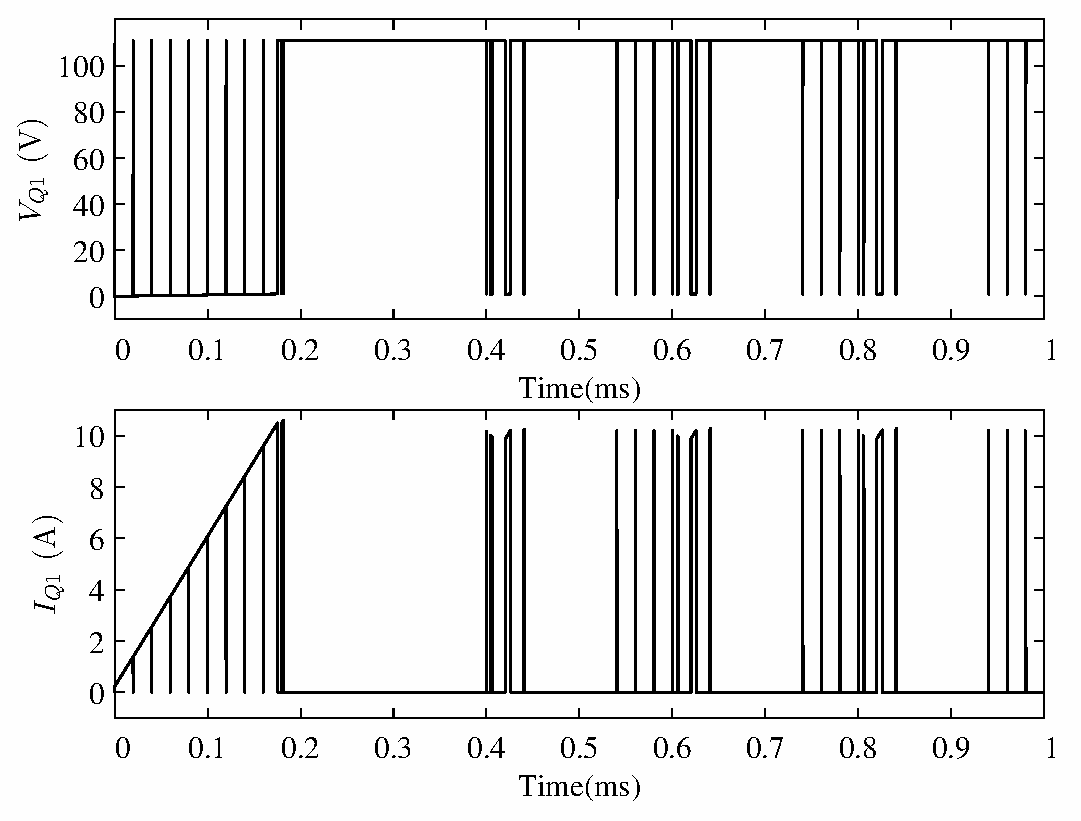
\includegraphics[width=0.95\linewidth]{Q1}
				\caption{Voltage and current of Q1}
				\label{fig:sim-q1}
			\end{subfigure}
			\begin{subfigure}{0.49\textwidth}
				\centering
				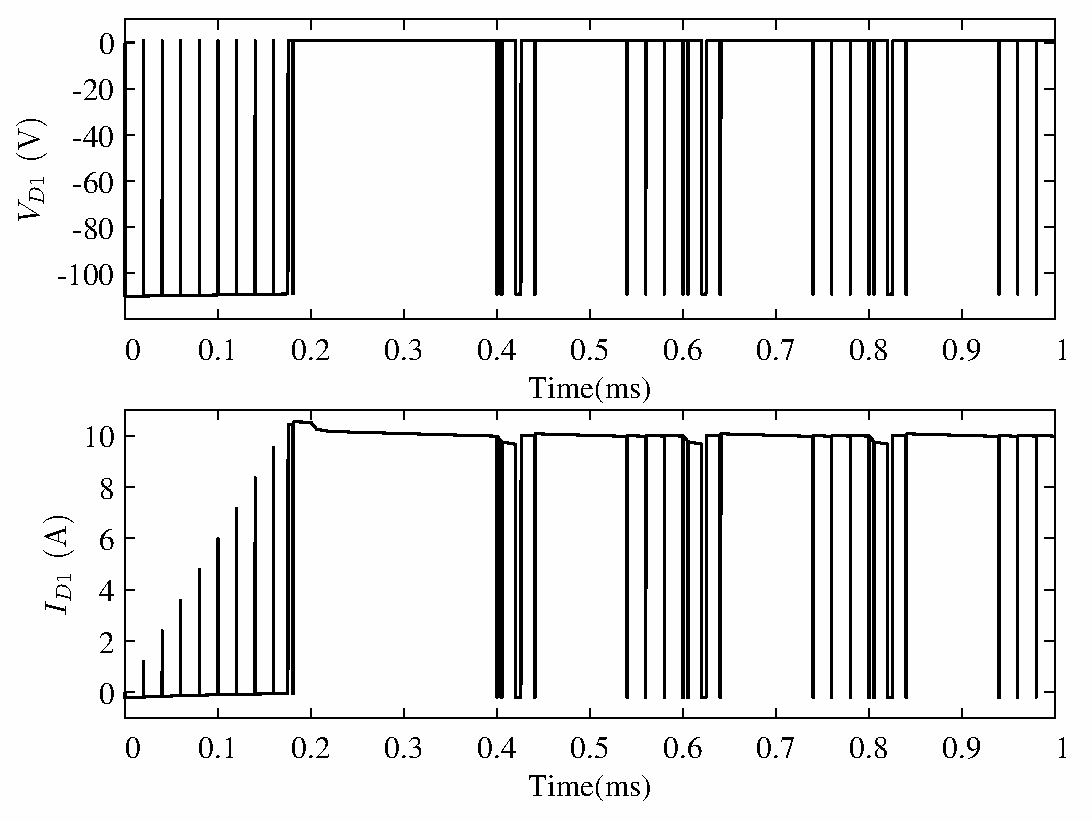
\includegraphics[width=0.95\linewidth]{D1}
				\caption{Voltage and current of D1}
				\label{fig:sim-d1}
			\end{subfigure}
			\caption{Direct duty ratio control: Q1,D1}
		\end{figure}
		Figure \ref{fig:sim-q2} shows the voltage across $Q_2$ and current through $Q_2$ waveforms when direct duty ratio control is used. The maximum voltage across $Q_2$ is $V_d$ i.e 110 V and the maximum current through it is 21 A. This maximum occurs during the rise time of the voltage source. Figure \ref{fig:sim-d2} shows the voltage across $D_2$ and current through $D_2$ waveforms when direct duty ratio control is used. The maximum reverse voltage across $D_2$ is $V_d$ i.e. 110 V and the maximum current through it is 4.5 A.
		\begin{figure}[H]
			\begin{subfigure}{0.49\textwidth}
				\centering
				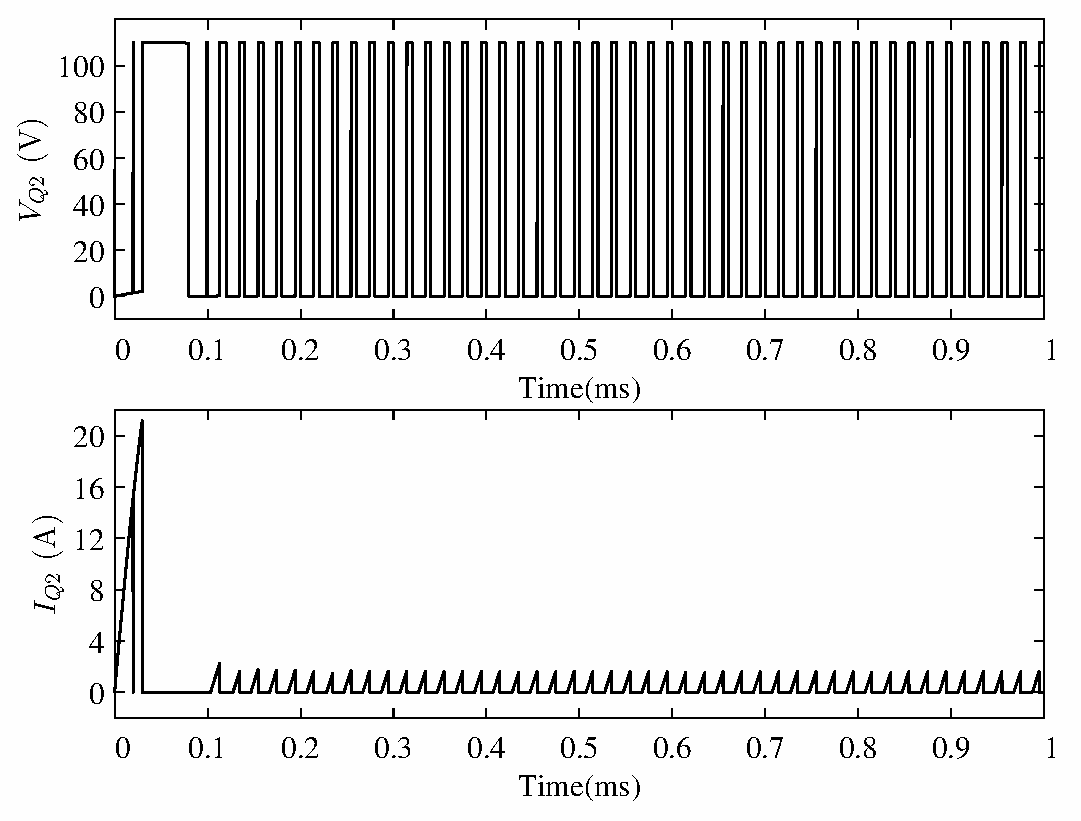
\includegraphics[width=0.95\linewidth]{Q2}
				\caption{Voltage and current of Q2}
				\label{fig:sim-q2}
			\end{subfigure}
			\begin{subfigure}{0.49\textwidth}
				\centering
				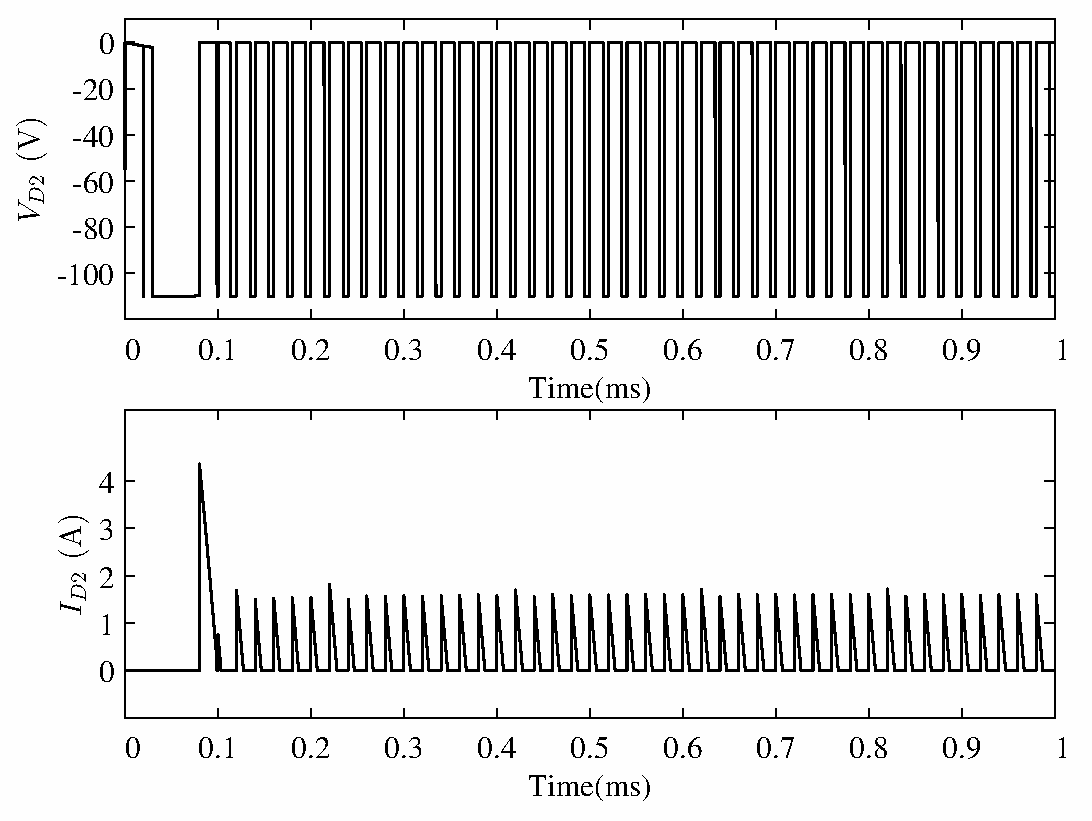
\includegraphics[width=0.95\linewidth]{D2}
				\caption{Voltage and current of D2}
				\label{fig:sim-d2}
			\end{subfigure}
			\caption{Direct duty ratio control: Q2,D2}
		\end{figure}
		Figure \ref{fig:sim-q3} shows the voltage across $Q_3$ and current through $Q_3$ waveforms when direct duty ratio control is used. The maximum voltage across $Q_3$ is 110 V and the maximum current through it is 4.5 A. Figure \ref{fig:sim-d3} shows the voltage across $D_3$ and current through $D_3$ waveforms when direct duty ratio control is used. The maximum reverse voltage across $D_3$ is 110 V and the maximum current through it is 21 A.
		\begin{figure}[H]
			\begin{subfigure}{0.49\textwidth}
				\centering
				\includegraphics[width=0.95\linewidth]{Q3}
				\caption{Voltage and current of Q3}
				\label{fig:sim-q3}
			\end{subfigure}
			\begin{subfigure}{0.49\textwidth}
				\centering
				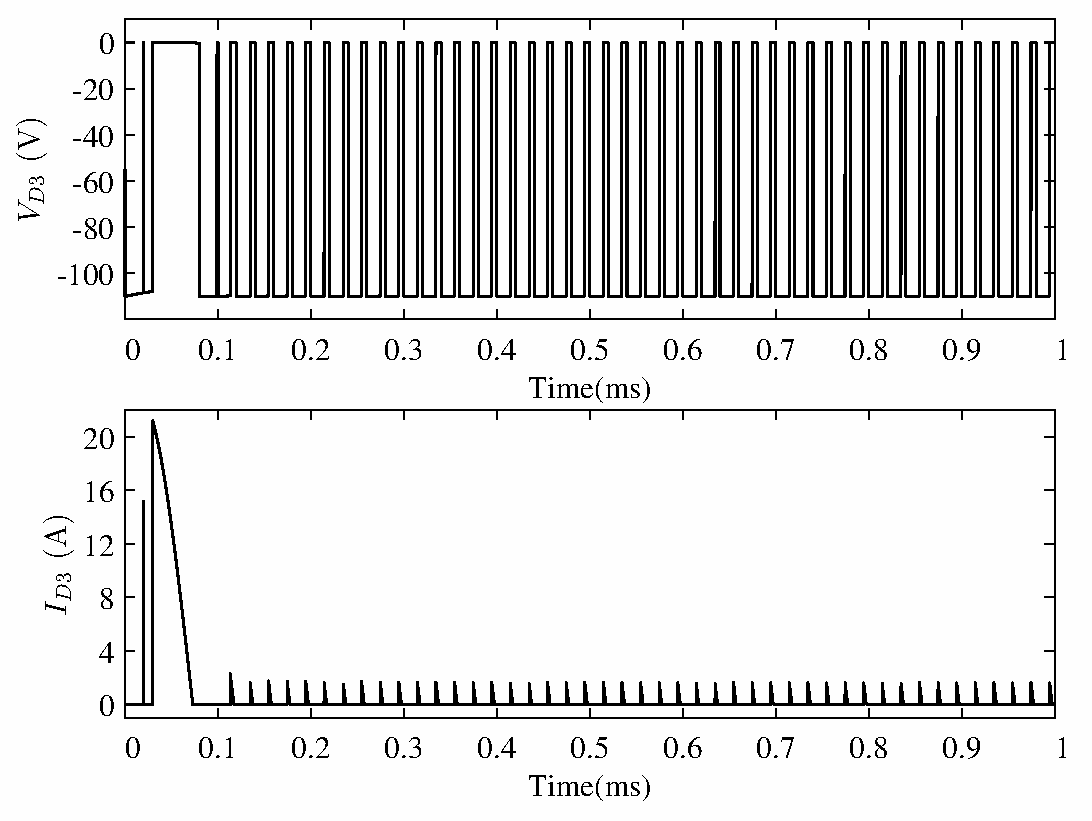
\includegraphics[width=0.95\linewidth]{D3}
				\caption{Voltage and current of D3}
				\label{fig:sim-d3}
			\end{subfigure}
			\caption{Direct duty ratio control: Q3,D3}
		\end{figure}
	\end{comment}
	\begin{table}[H]
		\centering
			\begin{tabular}{|l|l|} \hline
				Current source inductor & 2 mH \\ \hline
				Voltage source inductor & 100 $\mu$H \\ \hline
				Voltage source capacitor & 100 $\mu$F \\ \hline
				Switching frequency & 50 kHz \\ \hline
				Machining frequency & 5 kHz at 10\% duty \\ \hline
				DC link voltage & 110 V \\ \hline
				Current reference & 10 A \\ \hline
				Voltage reference & 80 V \\ \hline
				Load resistance & 1 $\Omega$ \\ \hline
			\end{tabular}
		\caption{Simulation parameters}
		\label{tab:sim1-param}
	\end{table}
\subsection{PI Control}
	\begin{figure}[H]
		\centering
		\includegraphics[width=0.6\textwidth]{results_2mh_pi}
		\caption{Load voltage and current: PI control}
		\label{fig:results_2mh_pi}
	\end{figure}
	Figure \ref{fig:results_2mh_pi} shows the load voltage and the load current when both the converters are controlled by PI controllers. The output waveforms thus obtained are similar to the results in \cite{tastekin2009novel}. The voltage source output is shown in figure \ref{fig:vs_2mh_pi} and the current source output is shown in figure \ref{fig:cs_2mh_pi}. The responses of both the sources are overdamped and their rise times are below 0.5 ms.
	\begin{figure}[H]
		\centering
		\begin{subfigure}{0.49\linewidth}
			\includegraphics[width=\linewidth]{cs_2mh_pi}
			\caption{Voltage source output}
			\label{fig:cs_2mh_pi}
		\end{subfigure}
		\begin{subfigure}{0.49\linewidth}
			\includegraphics[width=\linewidth]{vs_2mh_pi}
			\caption{Current source output}
			\label{fig:vs_2mh_pi}
		\end{subfigure}
		\caption{PI control}
	\end{figure}
	table \ref{tab:power} summarises the observed power consumption during the operation under constant reference as well as pulsed reference for the current source. The majority of the power is lost in $r_L, Q_d, D_1$ as the machining duty for the WEDM process is very low.
	\begin{table}[H]
		\centering
		\begin{tabular}{|c|c|c|} \hline
			\textbf{Component} & \textbf{Power (Const. ref.)} & \textbf{Power (Pulsed ref.)} \\ \hline
			Source & 24.81 W & 11.99 W \\ \hline
			Load & 7.34 W & 7.34 W \\ \hline
			$r_L, Q_d, D_1$ & 16.47 W & 3.82 W \\ \hline
			Other & 1.06 W & 0.83 W \\ \hline
		\end{tabular}
		\caption{Power consumption for pulsed reference scheme}
		\label{tab:power}
	\end{table}

\subsection{Current Mode Control}
	\begin{figure}[H]
		\centering
		\includegraphics[width=0.6\textwidth]{results_2mh_cmc}
		\caption{Load voltage and current: Current mode control}
		\label{fig:results_2mh_cmc}
	\end{figure}
	Figure \ref{fig:results_2mh_cmc} shows the load voltage and the load current when both the converters are controlled via current mode control. While the load voltage and current are similar to the PI controller, the the response of voltage source is underdamped. The settling times of the voltage source is about 1 s while that of the current source is same as the previous. The voltage source output is shown in figure \ref{fig:vs_2mh_cmc} and the current source output is shown in figure \ref{fig:cs_2mh_cmc}.
	\begin{figure}[H]
		\centering
		\begin{subfigure}{0.49\linewidth}
			\includegraphics[width=\linewidth]{cs_2mh_cmc}
			\caption{Voltage source output}
			\label{fig:cs_2mh_cmc}
		\end{subfigure}
		\begin{subfigure}{0.49\linewidth}
			\includegraphics[width=\linewidth]{vs_2mh_cmc}
			\caption{Current source output}
			\label{fig:vs_2mh_cmc}
		\end{subfigure}
		\caption{Current mode control}
	\end{figure}
\subsection{Compensator Based Control}
	\begin{figure}[H]
		\centering
		\includegraphics[width=0.6\textwidth]{results_2mh_comp}
		\caption{Load voltage and current: Compensators}
		\label{fig:results_2mh_comp}
	\end{figure}
	Figure \ref{fig:results_2mh_pi} shows the load voltage and the load current when both the converters are controlled by lead-lag compensators. The voltage source output is shown in figure \ref{fig:vs_2mh_comp} and the current source output is shown in figure \ref{fig:cs_2mh_comp}. The current source is underdamped while the voltage source is overdamped with a significant settling time of 4 s. Several notches are present in the current source output during the pre-breakdown stages of the machining. However, there is no observable deviation from the expected load current and voltage. These are also observable in the hardware experiments and the possible causes are summarised later in this chapter.
	\begin{figure}[H]
		\centering
		\begin{subfigure}{0.49\linewidth}
			\includegraphics[width=\linewidth]{cs_2mh_comp}
			\caption{Voltage source output}
			\label{fig:cs_2mh_comp}
		\end{subfigure}
		\begin{subfigure}{0.49\linewidth}
			\includegraphics[width=\linewidth]{vs_2mh_comp}
			\caption{Current source output}
			\label{fig:vs_2mh_comp}
		\end{subfigure}
		\caption{Compensator based control}
	\end{figure}
	
\section{Hardware Experiments}
	\begin{figure}[h]
		\centering
		\begin{subfigure}{0.49\linewidth}
			
\includegraphics[width=\linewidth]{hardware-expt1}
			\caption{Operation with fixed resistance}
			\label{fig:hardware-expt1}
		\end{subfigure}
		\begin{subfigure}{0.49\linewidth}
			\includegraphics[width=\linewidth]{hardware-expt2}
			\caption{Operation with load switch}
			\label{fig:hardware-expt2}
		\end{subfigure}
		\caption{Hardware experiments}
	\end{figure}
	Table \ref{tab:hardware-param} summarises the specifications of the hardware setup which is used for experimentation. The operation of converter has been tested with a fixed load resistance as well as the combination of a resistance and switch. Figure \ref{fig:hardware-expt1} shows the load configuration for the first experiment where the current source is tested for disturbances. Another experiment has been carried out to test the converter in sparking like conditions. The load resistance is connected through the switch as shown in figure \ref{fig:hardware-expt2}.
	\begin{table}[h]
		\centering
			\begin{tabular}{|l|l|} \hline
				Current source inductor & 100$\mu$H \\ \hline
				Voltage source inductor & 2 mH \\ \hline
				Voltage source capacitor & 1000 $\mu$F \\ \hline
				Switching frequency & 50 kHz \\ \hline
				Machining frequency & 1 kHz at 50\% duty \\ \hline
				DC link voltage & 20 V \\ \hline
				Current reference & 4 A \\ \hline
				Voltage reference & 15 V \\ \hline
				Load resistance & 1 $\Omega$ \\ \hline
			\end{tabular}
		\caption{Experimental hardware specifications}
		\label{tab:hardware-param}
	\end{table}
	
\subsection{Operation With Fixed Load Resistance}
    The hardware setup developed in chapter \ref{chap:hardware} is used for initial experimentation with the converters. A load of 1 $\Omega$ is connected to the current controlled single quadrant converter. The ignition control switch is connected in parallel to this load to test for the response to disturbance to variable structure of the current source load. The current through the load resistor and the output voltage of the voltage controlled two quadrant converter is measured.
    \begin{figure}[H]
	    \begin{subfigure}{0.49\textwidth}
    		\centering
    		\includegraphics[width=0.95\linewidth]{switching-results}
    		\caption{Current Source switching test}
    		\label{fig:sw-results}
		\end{subfigure}
	    \begin{subfigure}{0.49\textwidth}
        	\centering
        	\includegraphics[width=0.95\linewidth]{transient}
    		\caption{Transient performance of current source}
    		\label{fig:transient}
		\end{subfigure}
		\caption{Current source performance under switching}
	\end{figure}
	Figure \ref{fig:sw-results} shows the current through the load resistor when ignition switch is operated at 1 kHz and the switching frequency of the converter itself is 100 kHz. The DC link voltage for this experiment is kept at 20 V. Voltage spikes corresponding to the ringing are observed in the current waveform. The transient performance of the current source under these conditions is shown in figure \ref{fig:transient}. It takes about 100 $\mu$s time for the current source to return to its normal operation after ignition switch is opened.
	\begin{comment}
	\begin{figure}[H]
		\centering
		\includegraphics[width=0.6\textwidth]{vsource-result}
		\caption{Voltage Source steady state performance}
		\label{fig:vsource-result}
	\end{figure}
	The steady state no load performance of the voltage source is shown in figure \ref{fig:vsource-result}. The conditions for this observations were same as the above.
	\end{comment}
	
\subsection{Operation With Load Switch}
	Figure \ref{fig:results} depicts the observed waveforms during complete operation of the converter. The ignition switch, which controls the machining duty is operated at 1kHz on 50\% duty while the switching frequencies of both the individual converters during this experiment is 50kHz. The load is a 1$\Omega$ resistance with a switch operating at 1kHz on 30\% duty to replicate the sparking phenomenon. The switching signals for the ignition switch and the load switch are on the top for comparison. The voltage and current are observed across the load terminals. The voltage across the diode D is also observed.
	
	When the ignition switch is opened, the diode D is forward biased and the voltage source output of 15V is reflected at the load terminals until the load switch is closed. Once the load switch is closed (representative of ignition of spark), the current is diverted through the load of 1$\Omega$ and the diode D is turned OFF. Hence, the voltage observed at the load terminals is the IR drop. When the ignition switch is closed, the current is diverted through the ignition switch which offers the lowest resistance path for the current flow and the voltage observed across the load terminals is the ON time voltage drop of the ignition switch. The current is allowed through the load only when the load switch is closed and its value during this period is the set reference of the current source.

	\begin{figure}[H]
		\centering
		\includegraphics[width=\textwidth]{results}
		\caption{Results}
		\label{fig:results}
	\end{figure}

	\begin{comment}
		\begin{figure}[H]
			\centering
			\includegraphics[width=0.6\textwidth]{results2}
			\caption{Hardware results for operation under switched R load}
			\label{fig:results2}
		\end{figure}
		The entire operation of the proposed converter relies on the fact that the voltage source output will appear across the spark gap terminals when the diode D is ON. To verify this, the above experiment has been run at the machining frequency of 100Hz to observer the behaviour of the converter under larger disturbance. It is observed that the load voltage follows the voltage source output when the D is ON. This is shown in figure \ref{fig:results2}.
	\end{comment}
	
	\begin{figure}[H]
		\centering
		\begin{subfigure}{0.49\textwidth}	
			\includegraphics[width=\linewidth]{l1current}
			\caption{Current source output}
			\label{fig:l1current}
		\end{subfigure}
		\begin{subfigure}{0.49\textwidth}
			\includegraphics[width=\linewidth]{c2voltage}
			\caption{Voltage source output}
			\label{fig:c2voltage}
		\end{subfigure}
		\caption{Individual converter performance under switched R load}
	\end{figure}
	
	Figure \ref{fig:c2voltage} shows the voltage source output i.e. the voltage across the voltage source capacitor. This voltage is equal to the reference voltage of 15 V. The current source output is shown in .For the current source, the inductor current is the output which is shown in figure \ref{fig:l1current}. This current is deviates from the expected output which should be a constant line of 4 A. The table \ref{tab:l1current} summarises the operation of the current source as observed in the second experiment.
	\begin{table}[H]
		\centering
		\begin{tabular}{|l|l|l|l|} \hline
		\textbf{Ref. in figure} & \textbf{Stage} & \textbf{Observation} & \textbf{Comments} \\ \hline
		1 & Sparking & $I_{L_1} \approx I_{ref}$ with some transients & Expected \\ \hline
		2 & Dead time & $I_{L_1} > I_{ref}$ & Not expected \\ \hline
		3 & Pre-breakdown & $I_{L_1} \approx 0$ A & Not expected \\ \hline
		\end{tabular} 
		\caption{Current source observations}
		\label{tab:l1current}
	\end{table}
	The load observed by the current source changes with the discharge stage, hence it is a Variable Structure System (VSS). The current source is tuned for fixed 1 $\Omega$ resistance load, therefore the current observed during the sparking stage is as expected. However, during the dead time, load seen by the current source is a short circuit condition. This condition offers least resistance path for the current causing the current to increase above the set reference. The linear controllers may not perform optimally for variable structured systems.
	
	The current dip during the pre-breakdown stage is result of low inductor value in the current source. This observation has been verified via simulations and the dip gets reduced for higher inductor values. This observation is consistent across the current mode control and the compensator based control. The energy stored in the inductor from the dead time is $1/2LI^2 = 0.125 mJ$, when the ignition switch is opened this energy is transferred to the capacitor via the decoupling diode. The voltage at the capacitor terminals increases according to the energy balance equation for this transfer.
	\begin{align*}
		\therefore \dfrac{1}{2}L(I_1^2 - I_2^2) &= \dfrac{1}{2}C(V_2^2 - V_1^2) \\
		\dfrac{1}{2}100\times 10^{-6}(5^2 - 0) &= \dfrac{1}{2}1000\times10^{-6}(V_2^2 - 15^2) \\
		V_2 &= 15.08 V
	\end{align*}
	Because the change in capacitor voltage is very small it is not observable from the output voltage waveforms. The entire energy stored in the inductor from the dead time is transferred to the voltage source capacitance causing only a small change in its voltage. As a result, the inductor current goes to zero.
	
	This means that the original assumption of current and voltage sources operating independently is not entirely true. The assumption is valid only when the inductor is large enough to cause a voltage disturbance which detectable and corrected by the voltage source. In the simulation results with a current source inductor of 2 mH, these voltage bumps are observed and handled by the voltage source. Thus, the current dips are lesser in the magnitude. Thus, the less inductor size and linear controller on VSS together cause the observed output current waveform. One possible solution to this issue is decreasing the voltage source capacitor as it is overrated for the present experimentation. The sliding mode controller can be used to maintain almost similar performance across all the VSS states.
\section{Conclusions}
\label{conclusions}
	A pulsed power supply has been developed for Wire Electric Discharge Machining application based on the original topology proposed by \citet{tastekin2009novel}. The this topology deviates from the standard DC-DC converter topologies leading to reduction in the damping factor as observed in the frequency responses in figure \ref{fig:uncomp-vs}. Moreover, due to these modifications standard ripple based sizing criteria is not adequate. Hence, the the appropriate values of L and C have inferred from the trajectories of the poles, which has been verified via the hardware setup.

	The ON state losses via the ignition switch dissipate power for about 70\% to 90\% of the time due to the low machining period requirement of the EDM process. These losses are reduced by lowering the current source reference during the dead time. The time averaging leads to only and approximate model of the converters. Hence, non linear model and sliding mode control has been designed and simulated for individual current and voltage sources each.
	
	The Semikron IGBT modules and the passive components have been assembled according to the topology mentioned in figure \ref{fig:working-3}.  PI controllers have implemented on a TI F28069 DSP board. The IGBTs are interfaced to the DSP via a buffer circuit. The operation of complete converter has been tested for DC link voltage of 20 to 50V at machining frequency of 1kHz.

	The current and voltage sensors with required range and bandwidth are not readily available. Hence, these sensors have been made using shunt resistance and potential dividers along with OP-AMP based conditioning circuits. The biases and slopes of the sensor response have been experimentally found out for their calibration.
	
	The voltage source used in the hardware is found to be working satisfactory but its output capacitor is overrated for the experimental conditions. The current source output had three distinct regions: (a) constant 4 A current region, (b) constant 5 A current region, and (c) zero current region. The possible reasons for these discrepancies have been identified which led to the conclusion that the current and voltage sources operate independently only for a sufficiently large current source inductor.

\section{Future Work}
\begin{itemize}
\item The sensors used in this work are based on resistances with 5\% tolerance band resulting in poor accuracy of the measurements. Moreover, the low power rating of these resistances limit operation to lower currents. This could be improved by using high precision measurement resistances.
\item The unexpected behaviour of the current source inductor as described in table \ref{tab:l1current} can be addressed by reducing the voltage source capacitor. Also, appropriate resizing of inductors and capacitors may be required for desired operation of the converter with an actual spark-gap load.
\item The pulsed reference scheme and sliding mode controller are illustrated with simulations only. The hardware implementation of the sliding mode controller can partially improve the current source inductor behaviour due its nonlinear nature.
\item The hardware experimentation has been done at reduced voltage and current levels. These levels have to be increased while experimenting with the spark-gap test cell.
\end{itemize}
	
\section{Publications}
The following paper is submitted based on the work done in this project.\\
M. Kane, \textbf{A. Khadse}, H. Bahirat, S. Kulkarni, ``Design and Control of Pulsed Voltage Supply for Electric Discharge Machining,'' in \textit{IEEE International Conference on Power Electronics, Drives and Energy Systems}, 2018 (Submitted)